\part{Transparency}
\frame{\partpage}

\begin{frame}{Alpha}
	\begin{itemize}
		\item We are used to working with colours in \textbf{RGB} space
		\pause\item We can also work in \textbf{RGBA} space, where A = alpha = transparency
		\pause\item $A=0 \implies$ fully transparent
		\pause\item $A=1$ (or $A=255$) $\implies$ fully opaque
	\end{itemize}
	\pause
	\begin{center}
		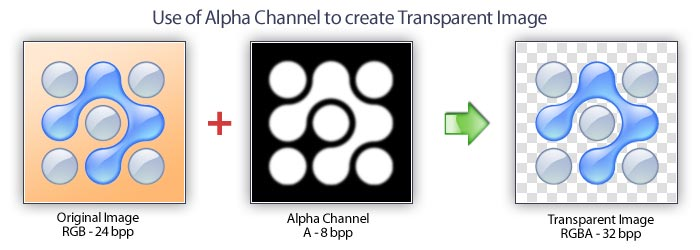
\includegraphics[width=\textwidth]{alpha_channel}
	\end{center}
\end{frame}

\begin{frame}[fragile]{Alpha in OpenGL}
	\begin{itemize}
		\item Use \lstinline[language=GLSL]{vec4} instead of \lstinline[language=GLSL]{vec3} for colours
		\pause\item Textures can have an \textbf{alpha channel}
			\begin{itemize}
				\pause\item PNG supports alpha channels, JPG and BMP do not
			\end{itemize}
		\pause\item Need to enable \textbf{alpha blending}
	\end{itemize}
	\pause
	\begin{lstlisting}
glEnable(GL_BLEND);
glBlendFunc(GL_SRC_ALPHA, GL_ONE_MINUS_SRC_ALPHA);
	\end{lstlisting}
	\begin{itemize}	
		\item Other values can be passed to \lstinline{glBlendFunc} for special effects
			(e.g.\ \textbf{additive blending} is often used for particle effects simulating
				light, fire, explosions etc.)
	\end{itemize}
\end{frame}

\begin{frame}{Transparency and depth testing}
	\begin{itemize}
		\item Recall we are using \textbf{depth testing}
			\begin{itemize}
				\pause\item Each fragment on screen remembers its \textbf{depth} (distance from the camera)
				\pause\item A new fragment is drawn \textbf{only if} its depth value is \textbf{less} than the current depth value
				\pause\item I.e.\ don't draw objects that should be behind something that was already drawn
			\end{itemize}
		\pause\item But if the object in front is (semi-)transparent, we want to see the object behind it!
		\pause\item Solution: draw semi-transparent objects \textbf{after} opaque objects,
			and in \textbf{back to front} order
		\pause\item Further discussion: {\footnotesize\url{http://www.opengl-tutorial.org/intermediate-tutorials/tutorial-10-transparency/}}
	\end{itemize}
\end{frame}
